\documentclass{beamer}
\usepackage{listings}
\lstset{
%language=C,
frame=single, 
breaklines=true,
columns=fullflexible
}
\usepackage{subcaption}
\usepackage{url}
\usepackage{tikz}
\usepackage{algorithm}
\usepackage{algorithmic}
\usepackage{tkz-euclide} % loads  TikZ and tkz-base
%\usetkzobj{all}
\usetikzlibrary{calc,math}
\usepackage{float}
\newcommand\norm[1]{\left\lVert#1\right\rVert}
\renewcommand{\vec}[1]{\mathbf{#1}}
\providecommand{\brak}[1]{\ensuremath{\left(#1\right)}}
\providecommand{\cbrak}[1]{\ensuremath{\{#1\}}}
\providecommand{\Mod}[1]{\ensuremath{\left\lvert#1\right\rvert}}
\usepackage[export]{adjustbox}
\usepackage[utf8]{inputenc}
\usepackage{amsmath}
\usetheme{Boadilla}
\usecolortheme{rose}

\title{Wireless Physical Layer Characteristics Based
Random Number Generator: Hijack Attackers}
\author{V.Samyuktha}
\institute{IITH}
\date{\today}
\begin{document}

\begin{frame}
\titlepage
\end{frame}

\begin{frame}{About the paper}
\begin{block}{Authors}
    \begin{itemize}
        \item Nin Gao
        \item Xiaojun Jing
        \item Shichao Lv
        \item Junsheng Mu
        \item Limin Sun
    \end{itemize}
\end{block}
\begin{block}{Abstract}
    \begin{itemize}
        \item Random numbers are widely used in 5G communication security. The most significant issue here is the generation of random numbers that are \textbf{unpredictable} and \textbf{reliable}.
        \item Proposed here is a wireless physical layer (PHY-layer) characteristics based random number generator in vehicular networks.
    \end{itemize}
\end{block}
\end{frame}

\begin{frame}{Why use PHY-layer?}
\begin{block}{Failure of traditional methods}
    \begin{itemize}
        \item Cannot prevent some attacks (eg: Jamming attacks)
        \item Heavy resource consumption, not suited for power limited networks.
    \end{itemize}
\end{block}
\begin{block}{Advantage of Physical Random Numbers Generator(PhRNG)}
    \begin{itemize}
        \item Utilize nondeterministic natural source as entropy to yield aperiodic and \textbf{true random numbers}. Hard to predict generator's output even if its design is known.
        \item No additional cost or complicated seed-generating algorithms.
    \end{itemize}
\end{block}
\end{frame}

\begin{frame}{Scenario}
\begin{block}{System model}
\begin{itemize}
    \item Vehicular network with two legitimate vehicles, where A is the initiator and B is the recipient.
    \item $K$ independent and identically distributed jamming attackers.
    \item Additional White Gaussian Noise(AWGN) with zero mean and variance $N_{0}$.
\end{itemize}
\end{block}
\begin{block}{Jamming attacks model}
\begin{itemize}
    \item Each attacks alternates between \textbf{sleeping} and \textbf{jamming} depending on time $t$.
    \item Jamming launch for time $t_{j}$ with constant power and then sleep for time $t_{s}$. Time $t=\cbrak{t_{j},t_{s}}$ can either be random and follow a distribution or be constant.
\end{itemize}
\end{block}
\end{frame}
\begin{frame}
\begin{block}{Formula for Recieved Signal}
    \begin{equation}
        R_{A,B}\brak{t}=\underbrace{\sqrt{P_{s}}h_{s}\brak{t}d_{s}}_{D_{s}} + \underbrace{\sqrt{P_{j}}\sum_{k=1}^{K}h_{k}\brak{t}d_{k}}_{I_{tot}} + n_{A,B}\brak{t}
    \end{equation}
    \end{block}
    Where,
    \begin{itemize}
        \item $h_{s}\brak{t}$ is the channel fading coeff. between A and B
        \item $h_{k}\brak{t}$ is the channel fading coeff. of the $k$-th jamming\
        \item $d_{s}$ is the unit energy desired signal
        \item $d_{k}$ is the $k$-th unit energy jamming signal
        \item $P_{s}$ is the desired signal energy
        \item $P_{j}$ is the energy of the jamming signal
        \item $n_{A,B}\brak{t}$ is the AWGN
    \end{itemize}
    Hence,
    \begin{itemize}
        \item $D_{s}$ is the desired signal
        \item $I_{tot}$ is the total of $K$ jamming attackers' signals
    \end{itemize}
\end{frame}
\begin{frame}{Physical Random Number Generator}
To arrive at the working of the proposed Random Transmission Success Probability based Physical Random Number Generator (RTSP-PhRNG) and describe the algorithm, we will first go through the following:\\
\begin{itemize}
    \item PDF of Signal-to-Interference and Noise Ratio(SINR)
    \item Random Transmission Success Probability(RTSP)
    \item Transform Theorem
    \item The complete algorithm
\end{itemize}
\end{frame}
\begin{frame}{PDF of SINR}
    SINR at B is given by:
    \begin{align}
        \nonumber\gamma &= \frac{P_{s}\Mod{h_{s}\brak{t}}^2\Mod{d_{s}}^2}{P_{j}\sum_{k=1}^{K}\Mod{h_{k}\brak{t}}^2\Mod{d_{k}}^2+N_{0}}\\
        \nonumber&= \frac{\Mod{D_{s}}^2/N_{0}}{\Mod{I_{tot}}^2/N_{0}+1}\\
        &= \frac{\gamma_{SN}}{\gamma_{IN}+1}\label{eq:2}
    \end{align}
    Where $\gamma_{SN}$ is the SNR power and $\gamma_{IN}$ is the sum of $K$ attackers' Intereference to Noise Ratio (INR) power. These variables follow gamma distribution.
\end{frame}
\begin{frame}{PDF of SINR}
    PDF of SNR power:
    \begin{equation}
        f_{SN}\brak{\gamma_{SN}} = \brak{\frac{m_{s}}{\Omega_{s}}}m_{s}\frac{\gamma_{SN}^{m_{s}-1}}{\Gamma\brak{m_{s}}}\exp\brak{-\frac{m_{s}}{\Omega_{s}}\gamma_{SN}}, \gamma_{SN}\geq{0}\label{eq:3}
    \end{equation}
    where $\Omega_{s}$ is the average SNR power and $m_{s}$ is the Nakagami-m fading parameter.\\
    If $k$-th INR power is given by: 
    \begin{equation}
        \nonumber\gamma_{IN,k} = P_{j}\Mod{h_{k}\brak{t}}^2\Mod{d_{k}}^2/N_{0}
    \end{equation}
    Then PDF of the $k$-th INR power is:
    \begin{equation}
         f_{IN}\brak{\gamma_{IN,k}} = \brak{\frac{m_{k}}{\Omega_{k}}}m_{k}\frac{\gamma_{IN,k}^{m_{k}-1}}{\Gamma\brak{m_{k}}}\exp\brak{-\frac{m_{k}}{\Omega_{k}}\gamma_{IN,k}}, \gamma_{IN,k}\geq{0}
    \end{equation}
\end{frame}
\begin{frame}{PDF of SINR}
    Adding up the $k$ different gamma distributions,
    \begin{equation}
        \nonumber\gamma_{IN} = \gamma_{IN,1} + \gamma_{IN,2} + ... + \gamma_{IN,k}
    \end{equation}
    Hence, the PDF of total INR power is given by:
    \begin{equation}
         f_{IN}\brak{\gamma_{IN}} = \brak{\frac{m_{i}}{\Omega_{i}}}m_{i}\frac{\gamma_{IN}^{m_{i}-1}}{\Gamma\brak{m_{i}}}\exp\brak{-\frac{m_{i}}{\Omega_{i}}\gamma_{IN}}, \gamma_{IN}\geq{0}\label{eq:5}
    \end{equation}
    where $\Omega_{i}$ is the average INR power and $m_{i}$ is the Nakagami-m fading parameter.\\
    Parameters $\Omega_{i}$ and $m_{i}$ are given by:
    \begin{equation}
        \Omega_{i}\approx\sum_{k=1}^{K}\Omega_{k}\text{ , } m_{i}\approx\frac{\brak{\sum_{k=1}^{K}\Omega_{k}}^2}{\sum_{k}^{2}/m_{k}}
    \end{equation}
\end{frame}

\begin{frame}{PDF of SINR}
    Quotient distribution of two random variables is given by:
    \begin{equation}
        f_{Z}\brak{z}=\int_{-\infty}^{\infty}f_{X}\brak{x}f_{Y}\brak{xz}\Mod{x}dx\nonumber
    \end{equation}
    Using this with \eqref{eq:2}, PDF of SINR at B is given by:
    \begin{equation}
        f_{SIN}\brak{\gamma} = \int_{1}^{+\infty}f_{IN}\brak{x-1}f_{SN}\brak{x\gamma}xdx, \gamma\geq{0}\label{eq:7}
    \end{equation}
    Substituting \eqref{eq:3} and \eqref{eq:5} into \eqref{eq:7}, and after solving the integral, we get:
    \begin{block}{Final equation for PDF of SINR}
    \begin{equation}
    \begin{split}
        f_{SIN}\brak{\gamma}&=\frac{\brak{\frac{m_{s}}{\Omega_{s}}}^{m_{s}}\brak{\frac{m_{i}}{\Omega_{i}}}^{m_{i}}\gamma^{m_{s}-1}\exp\brak{-\frac{m_{s}}{\Omega_{s}}\gamma}}{\Gamma\brak{m_{s}}}\\
        &\times
        \brak{\frac{m_{s}}{\Omega_{s}}\gamma+\frac{m_{i}}{\Omega_{i}}}^{-m_{i}}
        \sum_{m=0}^{m_{s}}\binom{m_{s}}{m}\frac{m_{i}^{\brak{m}}}{\brak{\frac{m_{s}}{\Omega_{s}}\gamma+\frac{m_{i}}{\Omega_{i}}}^{m}},\gamma\geq{0}
    \end{split}
    \end{equation}
    \end{block}
\end{frame}
\begin{frame}{Random Transmission Success Probability}
    Defined as a random variable that describes the \textbf{probability of achieving signal reception} by a desired receiver.\\
    It can be evaluated by a random threshold, $\gamma_{rv}$, and follows a Gaussian distribution.\\
    RTSP is given by:
    \begin{equation}
        P_{s}=\mathbb{P}\brak{SINR>\gamma_{rv}}\label{eq:13}
    \end{equation}
    Substituting for $f_{SIN}\brak{\gamma}$, and solving the integral, we get:
    \begin{block}{Final Expression for RTSP}
    \begin{equation}
    \begin{split}
        P_{s}&=\brak{\frac{m_{i}/\Omega_{i}}{\frac{m_{s}}{\Omega_{s}}\gamma_{rv}+\frac{m_{i}}{\Omega_{i}}}}^{m_{i}}\exp\brak{-\frac{m_{s}}{\Omega_{s}}\gamma_{rv}}\sum_{n=0}^{m_{s}-1}\\
        &\times\frac{\brak{m_{s}\gamma_{rv}/\Omega_{s}}^{n}}{n!}\sum_{m=0}^{n}\binom{n}{m}\frac{\brak{m_{i}}^{\brak{m}}}{\brak{\frac{m_{s}}{\Omega_{s}}\gamma_{rv}+\frac{m_{i}}{\Omega_{i}}}^{m}}
    \end{split}
    \end{equation}
    \end{block}
\end{frame}
\begin{frame}{Random Transmission Success Probability}
    \begin{itemize}
        \item We can see that RTSP is a function of the random variable $m_{s}\gamma_{rv}/\Omega_{s}$.
        \item It contains the PHY-layer characteristics such as average SNR power $\Omega_{s}$ and Nakagami-m fading parameter $m_{s}$. 
        \item According to the Transfer Theorem (explained next), \textbf{$P_{s}$ is a random variable distributed uniformly on $U\brak{0,1}$}.
    \end{itemize}
\end{frame}
\begin{frame}{Probability Integral Transform Theorem}
\begin{block}{Supporting Lemma}
    If a random variable $X$ has CDF $\mathbb{P}\brak{.}$. Then for all real $x$, $P\cbrak{\mathbb{P}\brak{X}\leq{\mathbb{P}\brak{x}}}=\mathbb{P}\brak{x}$
\end{block}
    \begin{block}{Statement}
        If the CDF $\mathbb{P}\brak{.}$ for a random variable $X$ is continuous, then a new random variable $Y=\mathbb{P}\brak{X}$ will be distributed uniformly on $U\brak{0,1}$.
    \end{block}    
    \begin{block}{Proof}
        Let $y\epsilon\brak{0,1}$, since $Y=\mathbb{P}\brak{X}$ and $\mathbb{P}\brak{.}$ is continuous, there must exist a real $x$ such that $\mathbb{P}\brak{X}=Y$.\\
        Then, $P\cbrak{Y\leq{y}}=P\cbrak{\mathbb{P}\brak{X}\leq{y}}=P\cbrak{\mathbb{P}\brak{X}\leq{\mathbb{P}\brak{x}}}=P\cbrak{X\leq{x}}=\mathbb{P}\brak{x}=y$.\\
        Hence, the random variable Y is uniformly distributed on $U\brak{0,1}$
    \end{block}
\end{frame}
\begin{frame}{Complete Algorithm}
    RTSP-PhRNG algorithm consists of \textbf{detection algorithm} and \textbf{generation algorithm}.
    \begin{block}{Detection algorithm} 
        Keep track of signal energy to detect random jamming attacks.
        The signal energy distribution evaluated by $N$ samples of the received signal $R\brak{t}$ in time slot $s$ is represented as
        \begin{equation}
            Y=\frac{1}{N}\brak{\sum_{s}^{s-N+1}R\brak{s}^{2}}
        \end{equation}
        The binary hypothesis test uses an energy threshold $\Theta$ that is chosen after considering tradeoffs between probability of detection and false alarm.
        \begin{align}
            H_{0} &: P\brak{D_{1}|Y}<\Theta,\nonumber\\
            H_{1} &: P\brak{D_{1}|Y}\geq{\Theta}.\label{eq:12}
        \end{align}
        $D_{1}$ represents attacker present and $Y$ represents the received signal energy.
    \end{block}
\end{frame}
\begin{frame}{Complete Algorithm}
    \begin{block}{Supporting Theorem}
        If a continuous random variable $X$ is distributed uniformly on $U\brak{0,1}$, the discrete random variable $Y$ which is discrete of $X$ by a quantization threshold $\lambda=1/2$, follows a binary uniform distribution $U_{b}\brak{0,1}$.
    \end{block}
    \begin{block}{Proof}
        Let \begin{equation}
            y=
            \begin{cases}
            1, &\text{for } x>\lambda\\
            0, &\text{for } x\leq{\lambda}
            \end{cases}
        \end{equation}
        Since $P\brak{Y=0}=\mathbb{P}\brak{X\leq{\lambda}}=\mathbb{P}\brak{X\leq{1/2}}=1/2$\\
        and $P\brak{Y=1}=\mathbb{P}\brak{X>{\lambda}}=1-\mathbb{P}\brak{X\leq{1/2}}=1/2$,\\
        the discrete random variable $Y$ follows a binary uniform distribution
        \begin{equation}
            P\brak{Y=y}=
            \begin{cases}
            1/2, &\text{for }y=1,\\
            1/2, &\text{for }y=0.
            \end{cases}
        \end{equation}
    \end{block}
\end{frame}
\begin{frame}{Complete Algorithm}
\begin{algorithm}[H]
\algsetup{linenosize=\tiny}
\scriptsize
\hspace*{\algorithmicindent} \textbf{Input:} \\
    \hspace*{\algorithmicindent} $A$'s Random Transmission Success Probability $P_{s}$\\
    \hspace*{\algorithmicindent} \textbf{Output:} \\
    \hspace*{\algorithmicindent} Binary random numbers $R\sim U\brak{0,1}$
\begin{algorithmic}[1]
\STATE Random jamming attackers detection using Eq.\eqref{eq:12}
\IF{state $H_0$}
    \STATE $A$ communicates with $B$ in communication mode.
\ELSE
    \STATE $A$ switches to PhRNG mode and generates random transmission success probability $P_{s}$
    \STATE Set quantization threshold $\lambda=1/2$
    \FOR{$j\longleftarrow1$ to length $\Mod{P_{s}}$}
        \IF{$P_{s}\brak{j}\geq \lambda$}
            \STATE $P_{s}\brak{j}=1$
        \ELSE
            \STATE $P_{s}\brak{j}=0$
        \ENDIF
        \STATE $R\brak{j}=P_{s}\brak{j}$
    \ENDFOR
    \STATE Return binary random numbers $R$
\ENDIF
\end{algorithmic}
\caption{RTSP-PhRNG}
\end{algorithm}
\end{frame}
\begin{frame}{Results and Simulation}
    \begin{figure}[!htb]
        \centering
        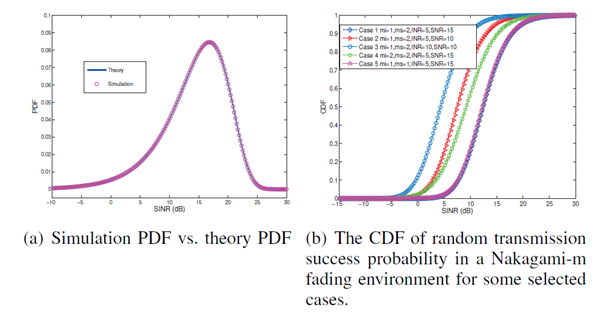
\includegraphics[width=0.8\columnwidth]{figure-1.png}
        \caption{Simulation Results}
        \label{fig:simulation}
    \end{figure}
In graph (a), simulation PDF is compared with theory PDF for fading parameter $m_{s}=2$, $m_{i}=1$, SNR $\Omega_{s}=25dB$, and INR $\Omega_{i}=11dB$, respectively. \\
In (b), we analyze the impact of $\Omega_{s}$ on generation performance.
\end{frame}
\begin{frame}{Results and Simulation}
    \begin{block}{Inference}
        \begin{itemize}
            \item Higher SNR leads to larger RTSP for the same threshold.
            \item Average INR power has a remarkable influence. Higher interference leads to lower RTSP.
            \item Different degrees of fading also have effect on the performance. 
        \end{itemize}
    \end{block}
\end{frame}
\begin{frame}{Experimental Results}
     \begin{figure}[!htb]
        \centering
        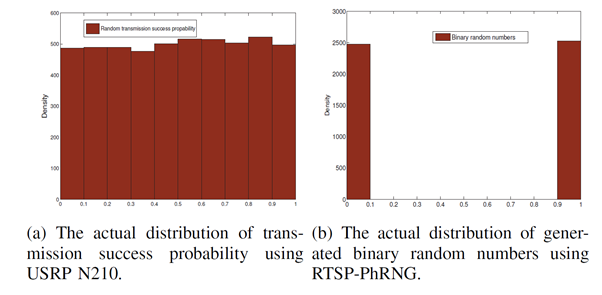
\includegraphics[width=0.75\columnwidth]{figure-2.png}
        \caption{Experiment Results}
        \label{fig:experiment}
    \end{figure}
    If $A$ sends out $n$ packets one time, but if only $m$ of them go, then RTSP is $m/n$. Random threshold $\gamma_{rv}$ is controlled by changing transmission power randomly (Gaussian random variable).\\
    $\lambda=1/2$ and packet rate = $25\times 10^3$ per second.\\
    The communicators and a jammer move in an indoor area randomly.
\end{frame}
\begin{frame}{Experimental Results}
    \begin{block}{Inference}
        \begin{itemize}
            \item The generated random numbers contain nearly the same number of $0$s and $1$s.
            \item Generation rate depends on packet rate and packet number $n$. (For this paper, max rate is 25 Kbps).
            \item Compared with Quantum random number generator and verified good effectiveness of result.
        \end{itemize}
    \end{block}
\end{frame}
\begin{frame}{Conclusion}
    \begin{block}{Final Points}
    \begin{itemize}
        \item A wireless PHY-layer characteristics based random numbers generator for vehicular networks has been proposed.
        \item Expression derived in terms of RTSP using a random threshold.
        \item Hijack the jamming attackers themselves.
        \item Effectiveness proved by simulation and results.
    \end{itemize}
    \end{block}
\end{frame}
\end{document}
